\chapter{Electric Motor}
\index{Electric Motor}

Electric motors are devices that convert electrical energy into mechanical energy. They operate
based on the interaction between magnetic fields and electric currents, producing rotational
motion. As mentioned previously, when an electric current flows through a conductor, it generates
a magnetic field around the conductor. If you place a magnet near this conductor, the
magnetic field will interact with the magnet's field, causing the conductor to experience a force.
This force can be harnessed to create motion, which is the fundamental principle behind electric motors.

\section{Basic Electric Motor}

The most common type of electric motor is the DC (Direct Current) brushed motor. It consists of a coil of wire
(armature) that rotates within a magnetic field created by permanent magnets or electromagnets. The armature 
is connected to a commutator, which reverses the direction of the current in the coil as it rotates, ensuring 
continuous rotation in one direction. The name "brushed" refers to the use of brushes that make contact with 
the commutator to supply current to the armature. 

TODO: Can there be a graphic of a basic electric motor? The generator image is similar, but the motor has a power source rather than a load.

Other types of electric motors include brushless DC motors, stepper motors, and AC (Alternating Current) motors. Each type has its own
characteristics and applications, but they all operate on the same basic principles of electromagnetism.

\section{Basic Electric Generator}
\index{Electric Motor ! Generator}

Electric generators are the reverse of electric motors. They convert mechanical energy into electrical energy by
using the principle of \newterm{electromagnetic induction}. When a conductor (such as a coil of wire) moves through a magnetic field, 
it induces an electric current in the conductor. This is covered in another chapter.

To construct a basic electric generator, all you need is an electric motor and a load.
\begin{figure}[htbp]
    \centering
    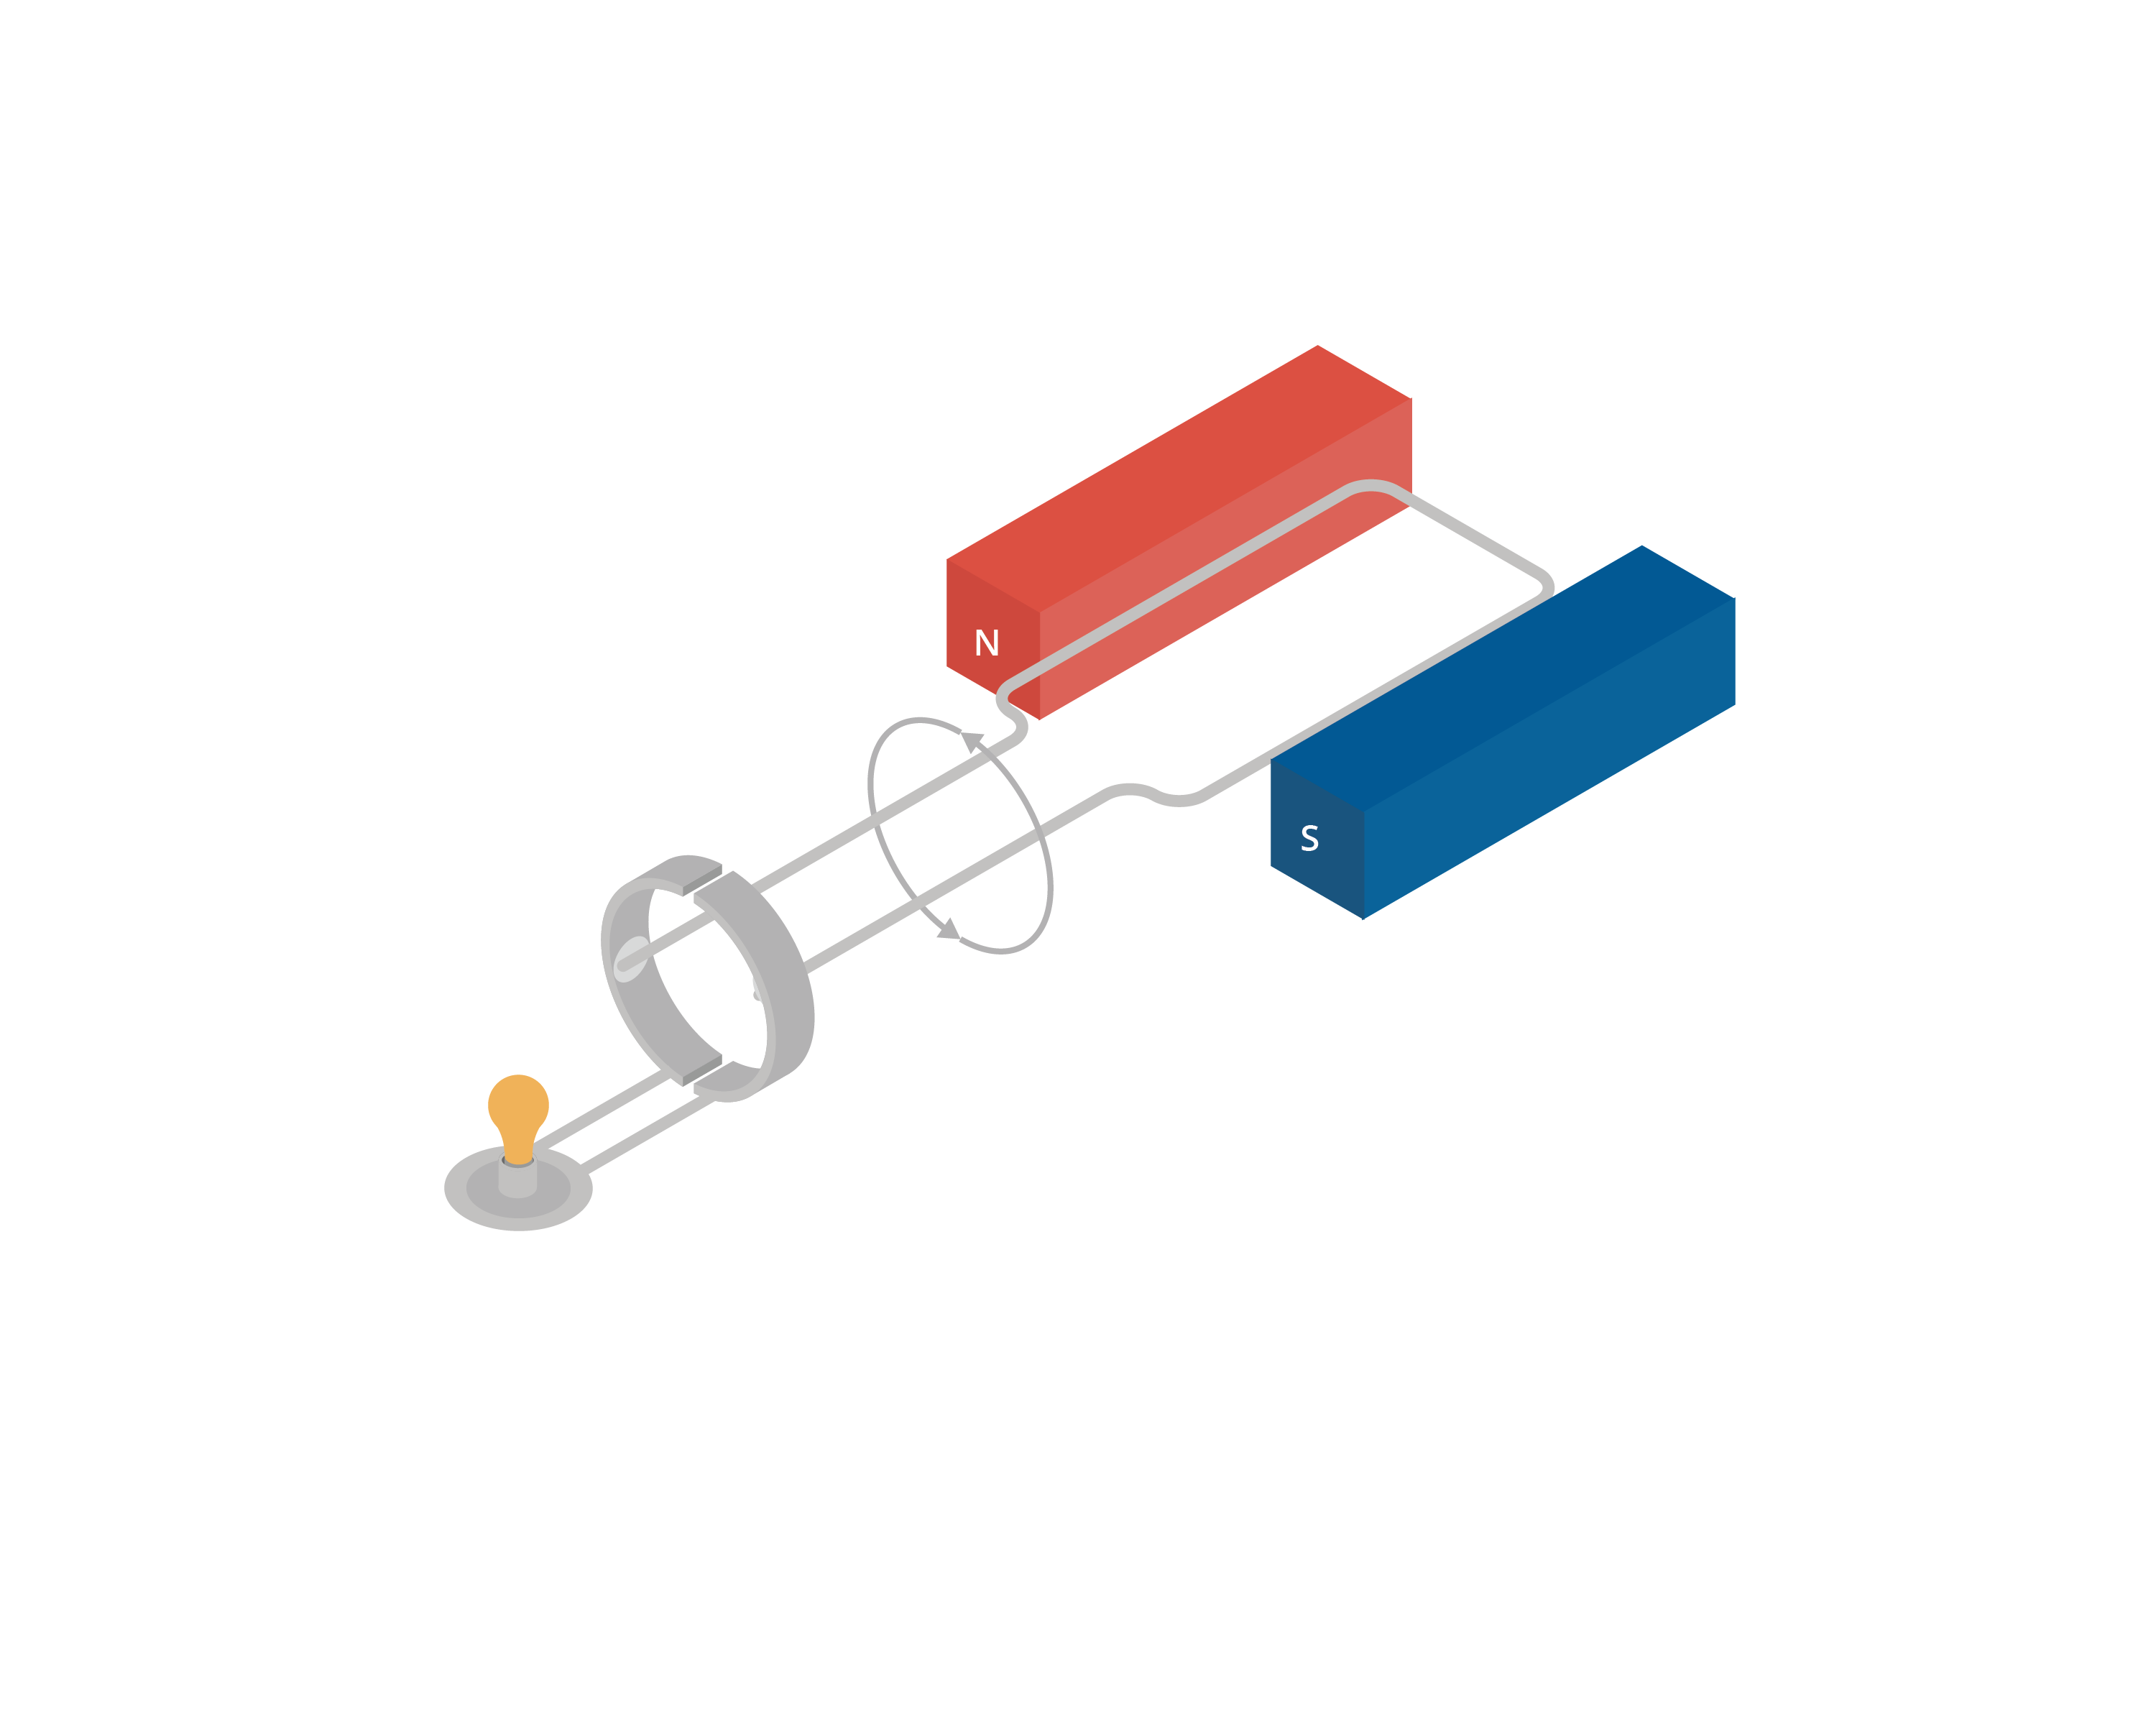
\includegraphics[width=0.75\textwidth]{basicGenerator.png}
    \caption{Basic Electric Generator Diagram}
    \label{fig:basic-generator-diagram}
\end{figure}

\clearpage

When you turn the motor with mechanical force, it will generate electricity that can be used to power a load. As the coil rotates within the 
magnetic field, the changing magnetic field induces a current in the coil, which can flow through the load, providing the necessary power. 

\begin{figure}[htbp]
    \centering
    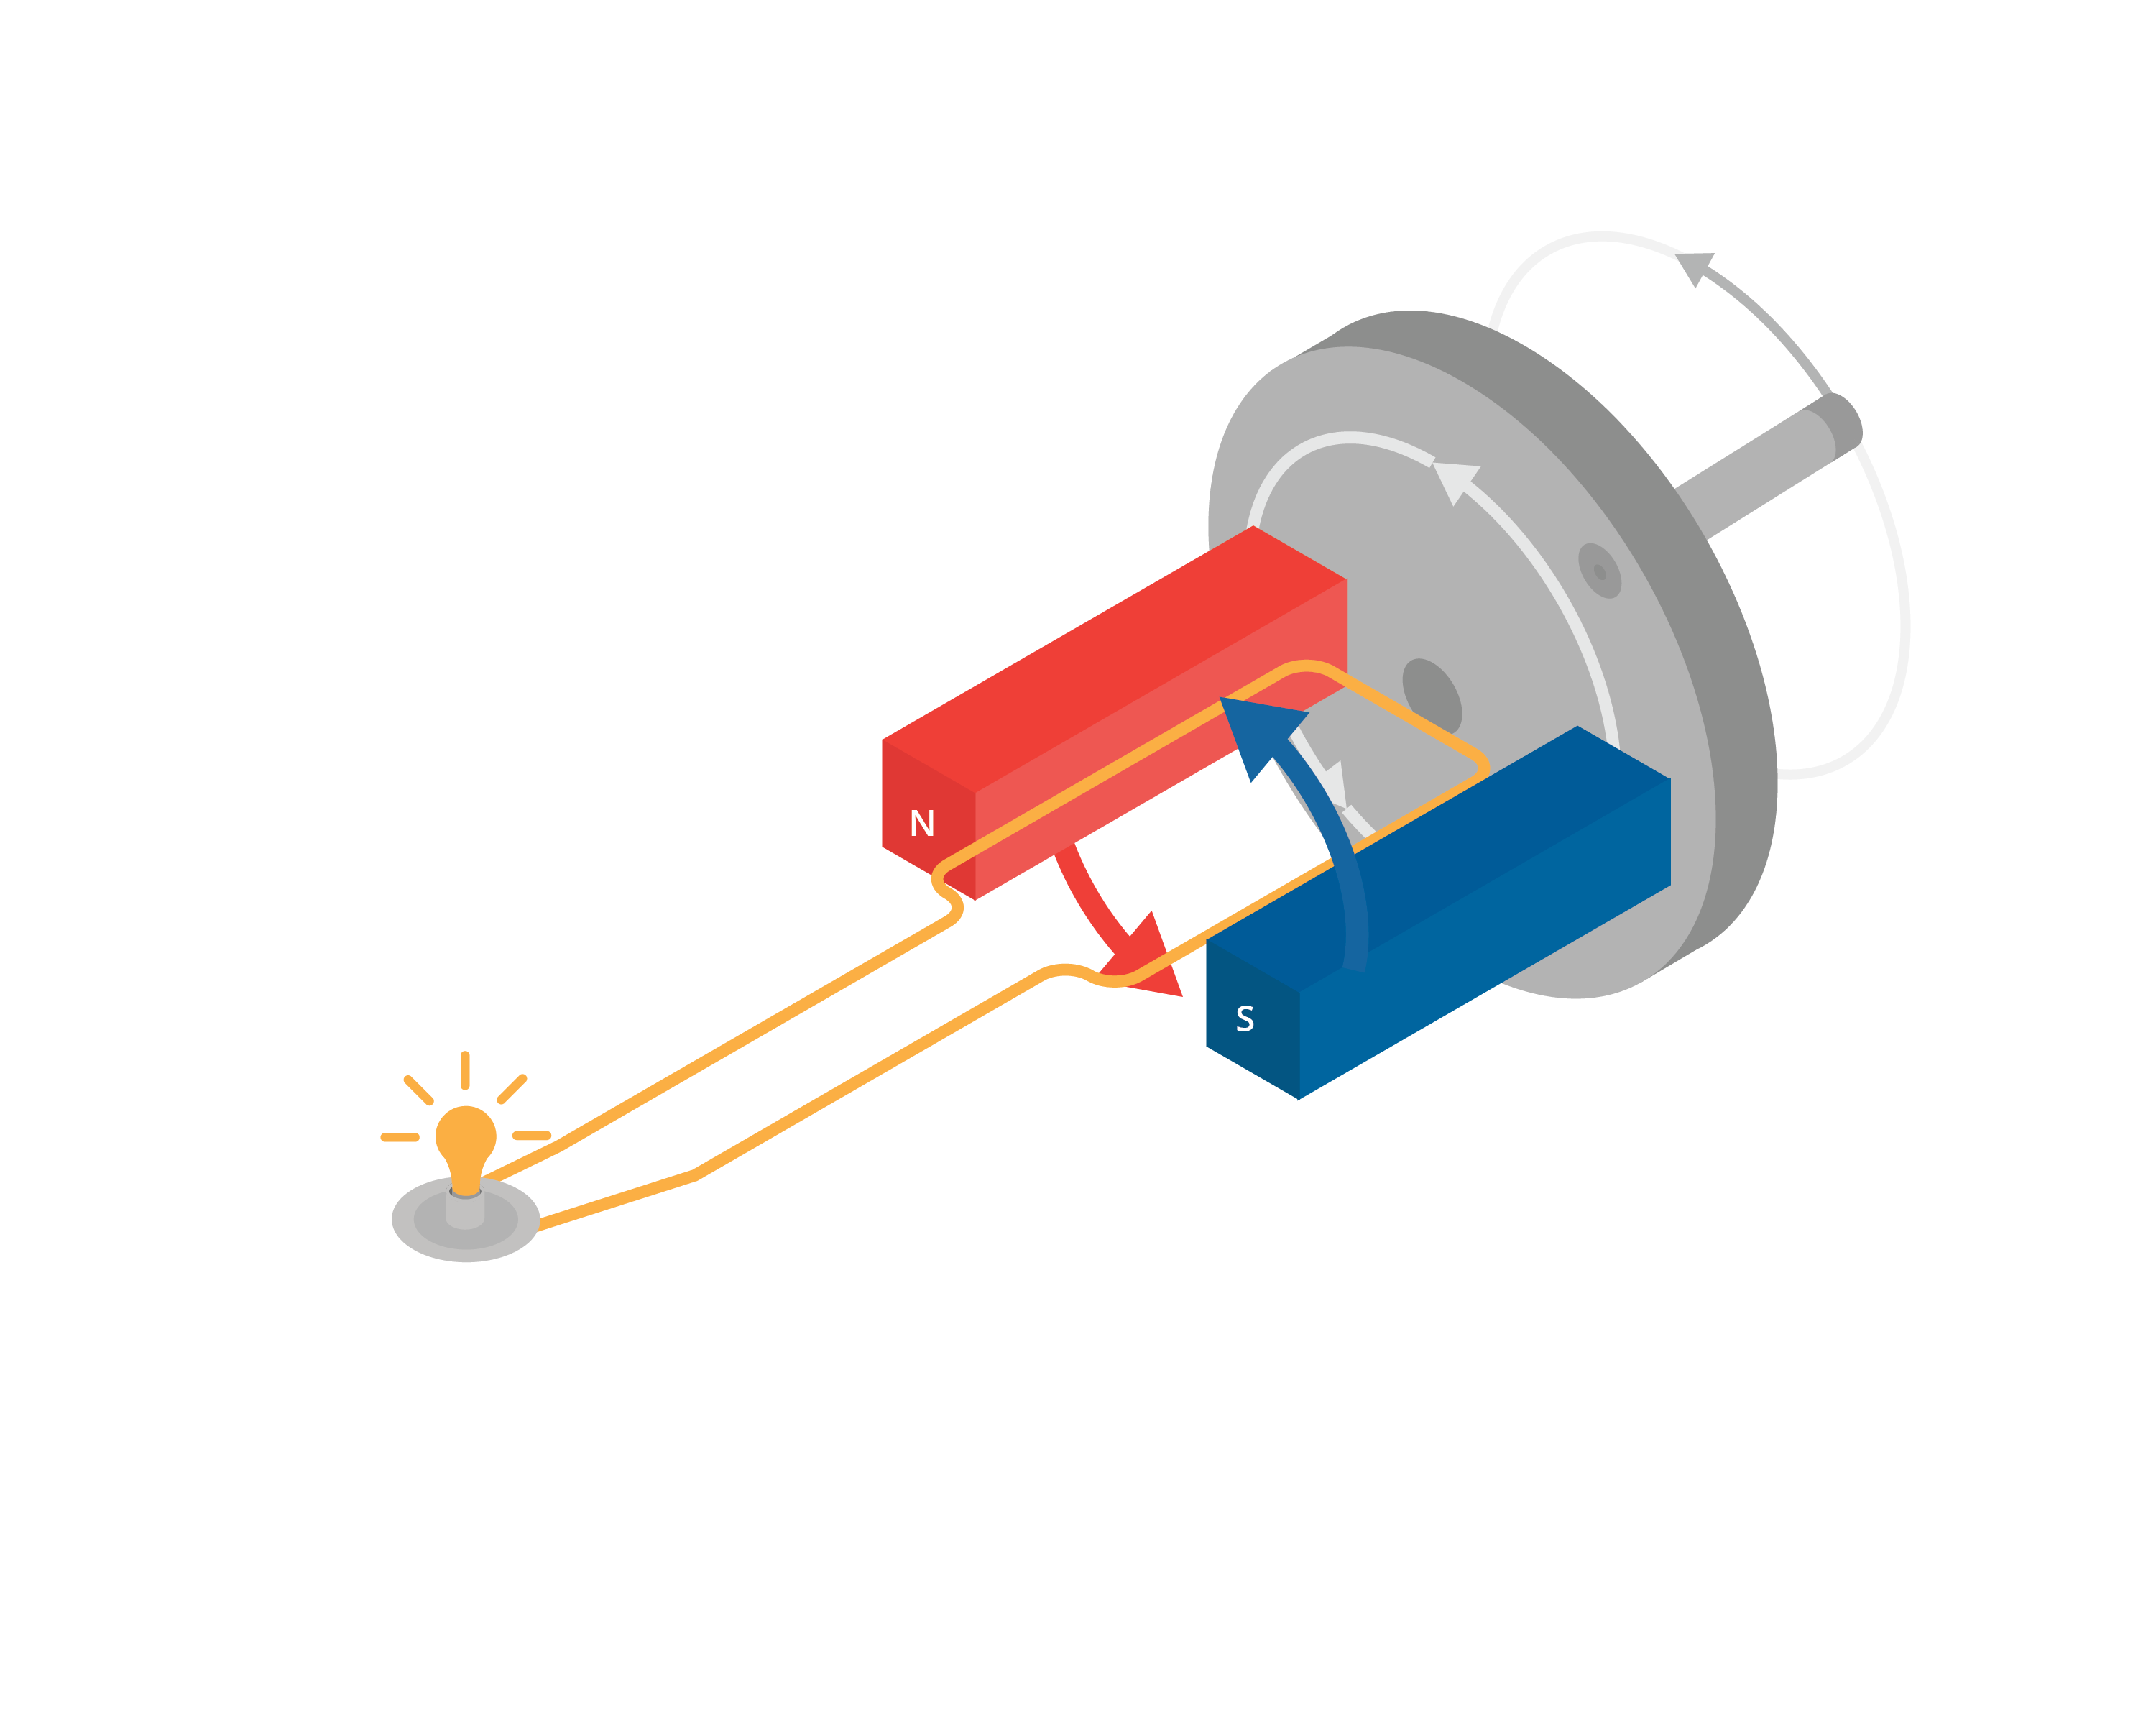
\includegraphics[width=0.35\textwidth]{basicGeneratorCrank.png}
    \caption{Basic Electric Generator in Motion with Handcrank}
    \label{fig:basic-generator-w-crank}
\end{figure}

If you instead turn the motor with a wheel, you can generate electricity in any manner of ways. This simple principle is used all
over the world to generate electricity. For example, in hydroelectric power plants, water is used to turn large turbines connected 
to generators, producing electricity on a massive scale. In wind power plants, wind turns the blades of a turbine, which is connected 
to a generator that produces electricity. In coal and natural gas power plants, steam is used to turn turbines connected to generators.

\begin{figure}[htbp]
    \centering
    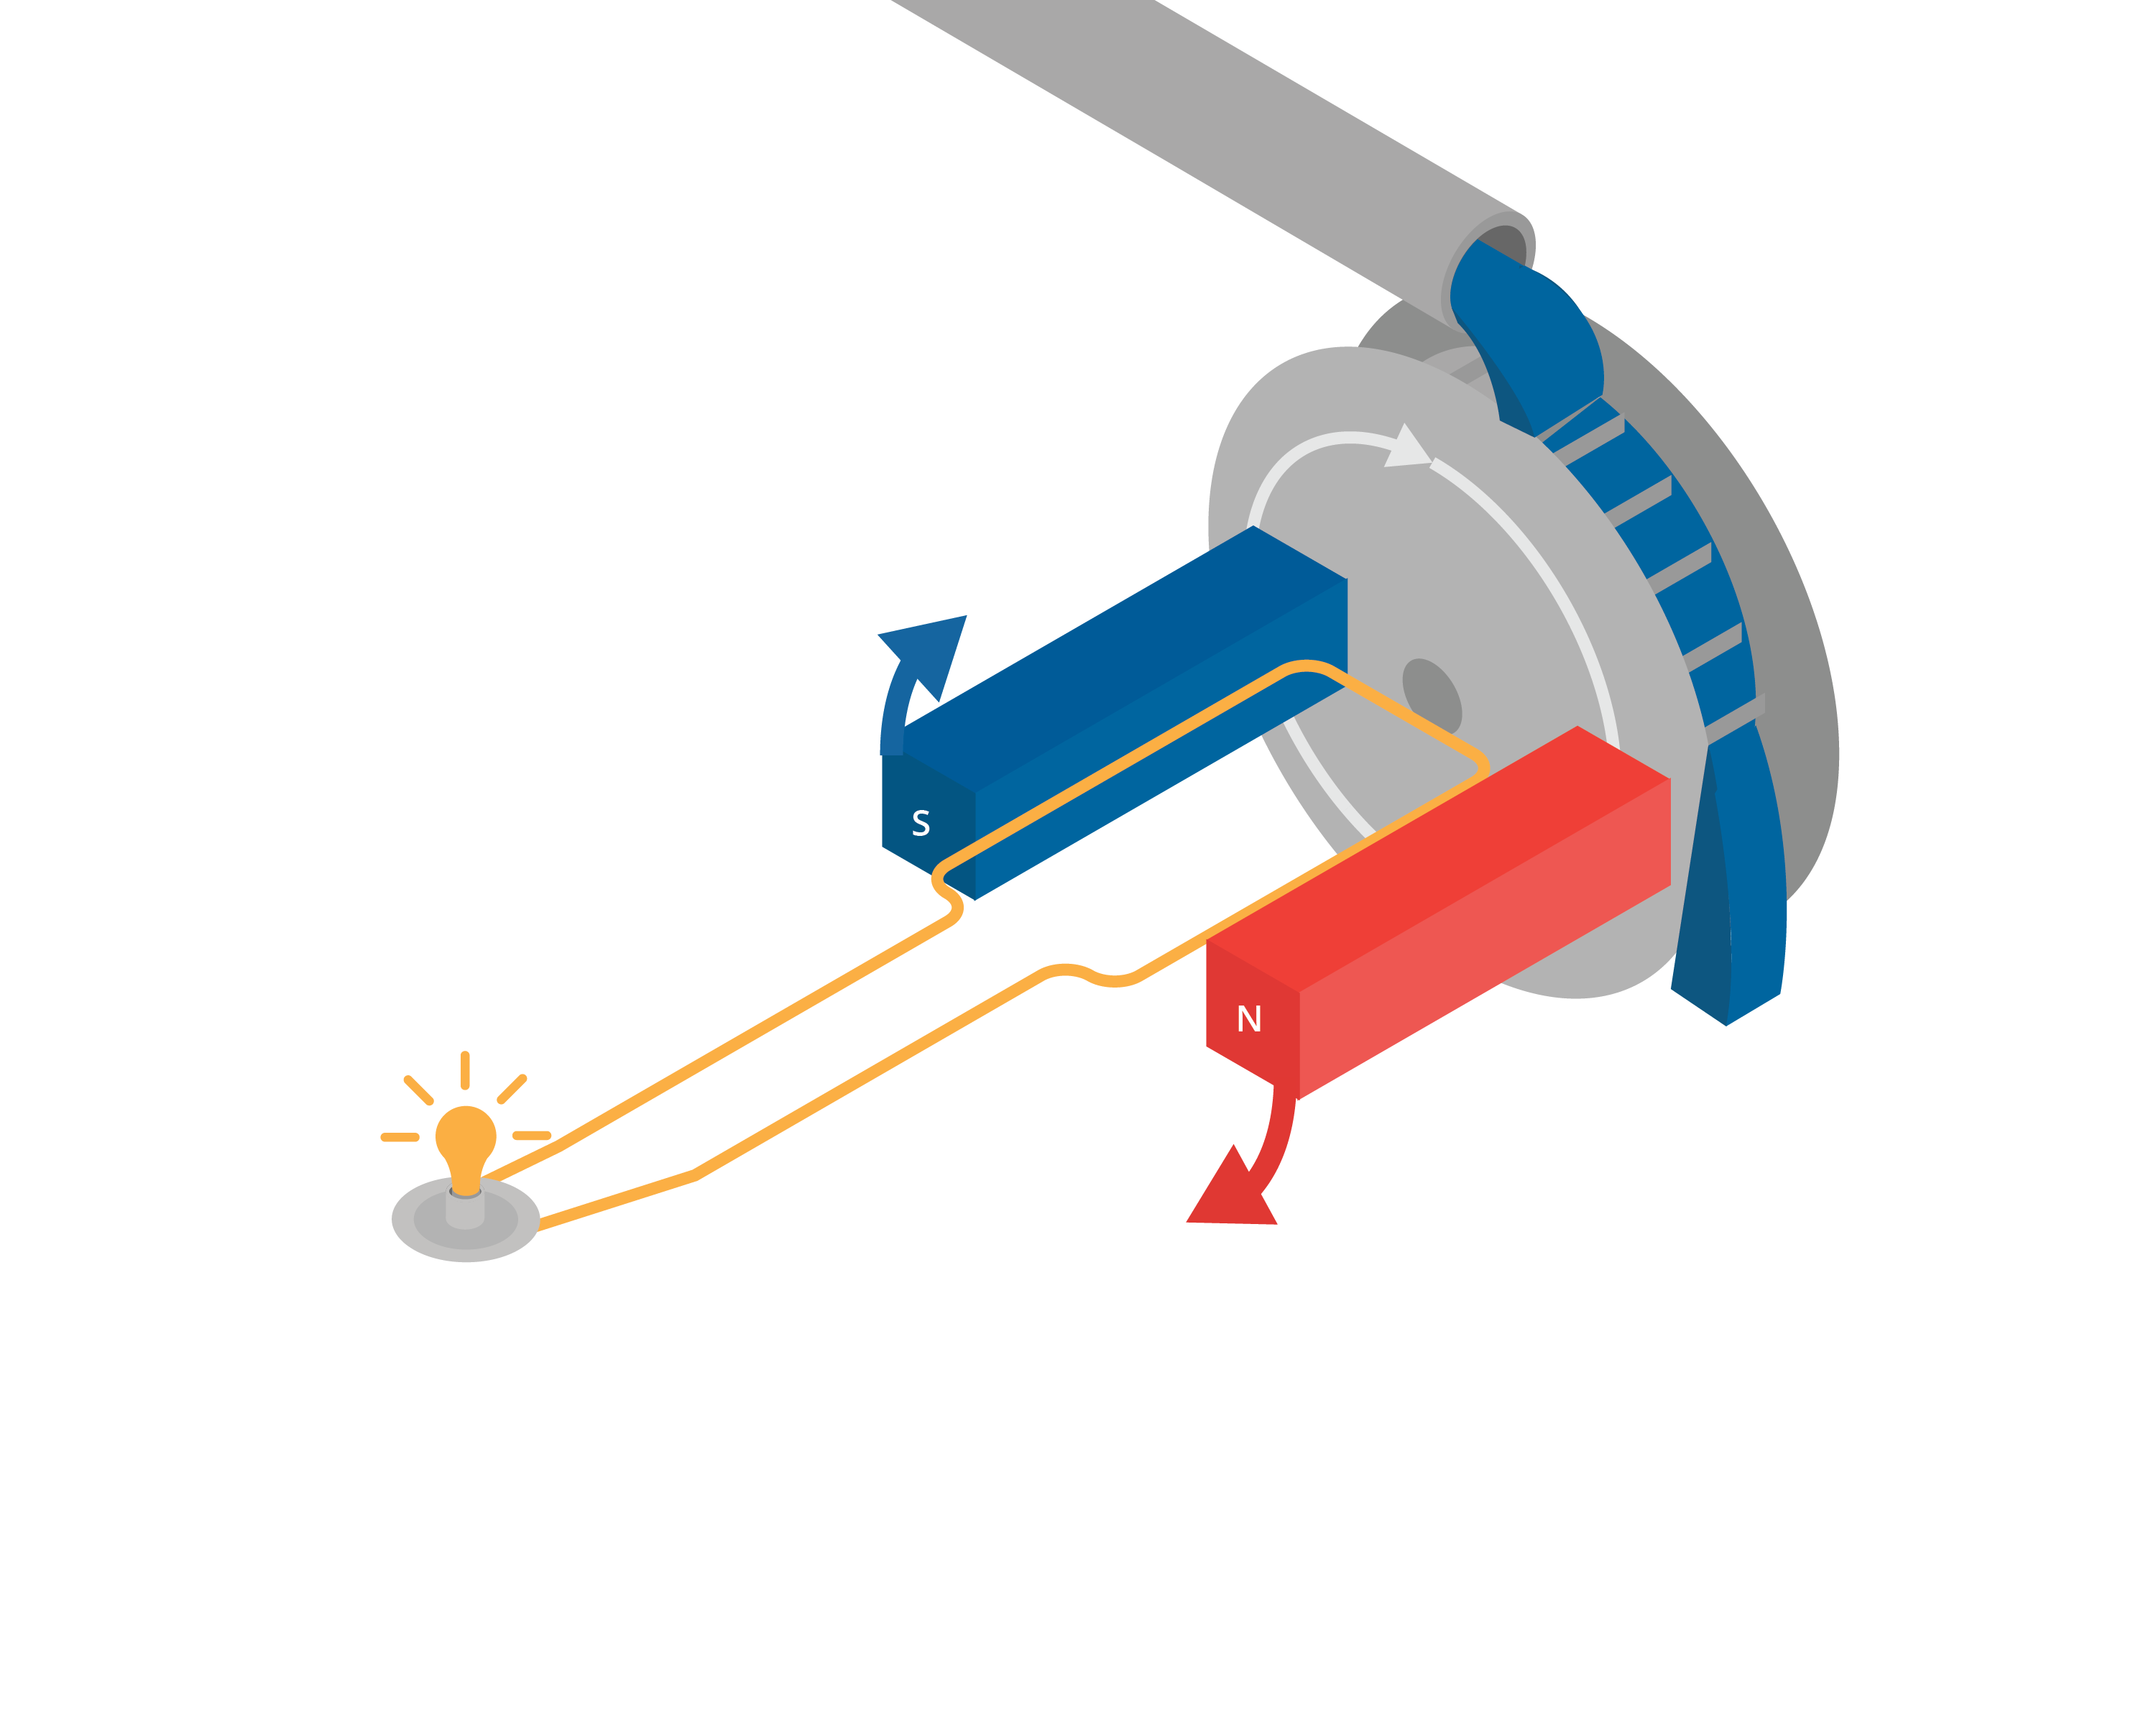
\includegraphics[width=0.35\textwidth]{basicGeneratorWheel.png}
    \caption{Basic Electric Generator in Motion with Wheel}
    \label{fig:basic-generator-w-wheel}
\end{figure}

